\vspace{-1pt}
\subsection{Path Pruning}
\label{method:3pathprune}

% \begin{figure*}[!t]
%     \centering
%     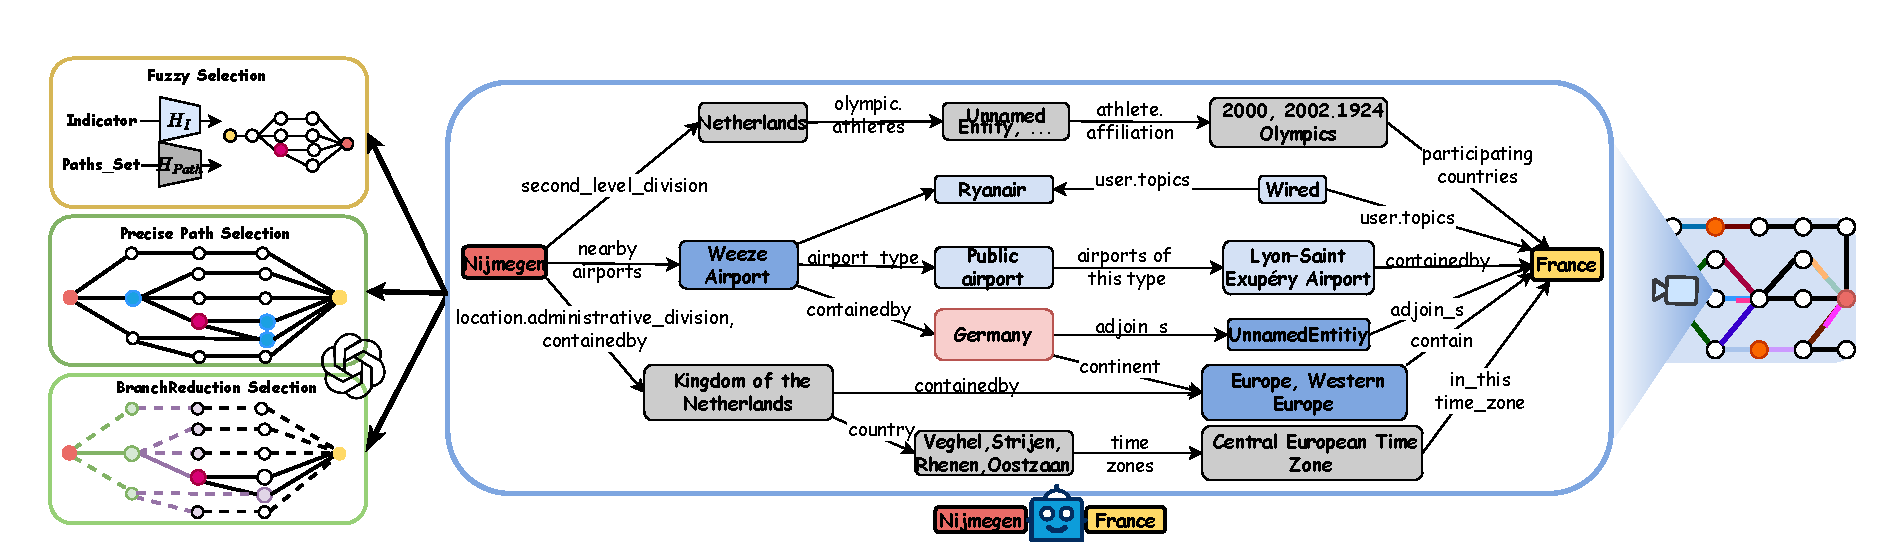
\includegraphics[width=\linewidth]{graphs/PathPrune.pdf}
%     \caption{The illustration of paths pruning.}

%     \vspace{-1em}
% \end{figure*}


As introduced in Section \ref{sec:related_work}, KGs contain vast amounts of facts,
making it impractical to involve all relevant triples in the LLM’s context due to high costs. To address this complexity and reduce LLM overhead, we utilize a three-step beam search for path pruning. The corresponding pseudo-code can be found in Appendix \ref{appendix:alg:pathpruning}.
% \subsubsection{Fuzzy Selection}

% \myparagraph{Fuzzy selection}
% Given the excessive volume of paths generated and the fact that only a small subset is likely relevant to the answer, the initial step in our beam search is fuzzy selection. This method is a non-LLM technique that aims to minimize additional computational overhead. For this purpose, we utilize SentenceBERT as a pruning tool to select the top-$W_1$ paths based on their literal similarities to the LLM indicator $I_{\text{LLM}}$.
% Specifically, we encode both the LLM indicator $I_{\text{LLM}}$ and all reasoning paths into dense vector embeddings. We then compute a cosine similarity matrix between these embeddings to determine their similarities. Ultimately, the paths with the highest top-$W_1$ similarity scores are selected for further processing. This step significantly reduces the number of paths that require evaluation by the LLM, thus lowering the overall computational demand.



\myparagraph{Fuzzy selection}
Considering that only a small subset of the generated paths is relevant,
the initial step of our beam search involves fuzzy selection by integrating a pre-trained language model (e.g. SentenceBERT \cite{reimers-gurevych-2019-sentence}), to filter the irrelevant paths quickly.
As shown in Figure \ref{fig:overall}, we encode the LLM indicator $I_{\text{LLM}}$ (or $I_{\text{Sup}}$) and all reasoning paths into vector embeddings, denoted as $H_I$ and $H_{Paths}$, and calculate cosine similarities between them. The top-$W_1$ paths with the highest similarity scores are  selected for further evaluation.
% \subsubsection{Precise Path Selection}

\myparagraph{Precise path selection}
Following the initial fuzzy selection, the number of candidate paths is reduced to $W_1$. At this stage, we prompt the LLM to select the top-$W_{\max}$ reasoning paths most likely to contain the correct answer. The specific prompt used to guide LLM in selection phase can be found in Appendix \ref{appendix:prompt}.

% \myparagraph{Branch reduced selection}
% Considering that the paths are represented in natural language and can sometimes be lengthy, resulting in high LLM processing costs, a branch reduction method by integrating the graph structure is utilized here to refine the path selection further. This method balances cost efficiency with accuracy in the final path selection.
% Starting from $D = 1$, for each entity in the entity list \ie $e\in list$, the method extracts the first $D$-step of $e$ from each path in the candidate set $Paths_c$ to the set $Paths_e$.
% If the number of $Paths_e$ exceeds the designated width $W_{max}$, these paths are pruned by precise path selection, and $Paths_c$ also be processed until the $|Paths_c| \leq D_{max}$.
% For example, in Figure \ref{fig:overall}, by setting $W_{max} = 1$, if we consider the red node only the first step is to extract the green paths, and the paths in dashed-line are pruned, for the next round, the path from orange to purple will be examed.
% Under the premise of ensuring the length and relevance of the reasoning path, Branch reduced selection achieves fast iterative selection with a small number of tokens.

% Based on the three path pruning methods, PoG supports various beam search strategies, ranging from non-reliant to fully reliant on LLMs, selectable in a user-friendly manner. We have defined the four strategies in Algorithm \ref{algorithm:PathsPruning}. 

\myparagraph{Branch reduced selection}
Considering that paths are often represented in natural language and can be extensive, leading to high processing costs for LLMs, we implement a branch reduced selection method integrated with the graph structure. This method effectively balances efficiency and accuracy by further refining path selection. Starting with $D = 1$, for each entity $e$ in the entity list, we extract the initial $D$-step paths from every path in the candidate set $Paths_c$ into a new set $Paths_e$. If the number of $Paths_e$ exceeds the maximum designated width $W_{\max}$, these paths are pruned using precise path selection. The process iterates until the number of paths in $Paths_c$ reaches $D_{\max}$. For example, as illustrated in Figure \ref{fig:overall}, with $W_{\max} = 1$, only the initial step paths (depicted in green) are extracted for further examination, while paths represented by dashed lines are pruned. This selection method enables efficient iterative selection by limiting the number of tokens and ensuring the relevance and conciseness of the reasoning paths.



\myparagraph{Beam search strategy}
Based on the three path pruning methods above,
% —fuzzy selection, precise path selection, and branch reduced selection—
PoG can support various beam search strategies, ranging from non-reliant to fully reliant on LLMs. These strategies are selectable in a user-friendly manner, allowing flexibility based on the specific requirements of the task. We have defined four such strategies in Algorithm \ref{algorithm:PathsPruning} of Appendix \ref{appendix:alg:pathpruning}. 



% \myparagraph{Branch Reduced Selection}
% Given that paths can be verbose and lead to high LLM processing costs, we implement a branch reduction method integrating graph structure to refine path selection efficiently. This method balances cost efficiency with accuracy in final path selection. The process starts with each entity $e \in \text{list}$, setting $D = 1$ to extract the first-step of $e$ from each path in the candidate set $Paths_c$ to the set $Paths_e$. If $Paths_e$ exceeds the designated width $W_{max}$, these paths undergo Precise Path Selection to narrow them down to $W_{max}$. Only selected $Paths_e$ and their corresponding original paths are retained; unselected paths are removed from $Paths_c$.

% If $Paths_c$ still exceeds $W_{max}$ after the first step, $D$ is incremented by one, and the process of extraction and selection repeats. This cycle continues until the quantity of $Paths_c$ aligns with width requirements. Ultimately, the refined $Paths_c$ are returned for further processing, ensuring that branch reduced selection achieves fast, iterative selection with minimal tokens.

% The three path pruning methods allow PoG to support various beam search strategies, ranging from non-reliant to fully reliant on LLMs, as outlined in Algorithm \ref{algorithm:PathsPruning}.
